\documentclass[manuscript]{aastex}
%-- Packages 
\usepackage[backref, breaklinks, colorlinks, citecolor=blue, linkcolor=magenta]{hyperref}
\usepackage[dvipsnames]{xcolor}

%\documentclass[]{emulateapj}
\newcommand{\vdag}{(v)^\dagger}
\newcommand{\myemail}{n.nicole.sanchez@vanderbilt.edu}

\slugcomment{Submitted to The Astrophysical Journal}

\shorttitle{Gas Accretion in MW-like Galaxies}
\shortauthors{N. N. Sanchez, J. M. Bellovary, \& K. Holley-Bockelmann}

\usepackage{natbib}
%\bibliographystyle{plain}
\bibliographystyle{apj}

\begin{document} 

\title{Cosmological Hydrodynamic Simulations of Preferential Accretion in the SMBH of Milky Way Size Galaxies}
%\title{A Particular Appetite: Cosmological Hydrodynamic Simulations of Preferential Accretion in the Supermassive Black Holes of Milky Way Size Galaxies}



\author{N. Nicole Sanchez \altaffilmark{1, 2}}
\author{Jillian M. Bellovary\altaffilmark{1, 2, 3}}
\author{Kelly Holley-Bockelmann\altaffilmark{1, 2}}

\affil{$^1$Fisk University, Nashville, TN, USA, n.nicole.sanchez@vanderbilt.edu}
\affil{$^2$Vanderbilt University, Nashville, TN, USA}
\affil{$^3$American Museum of Natural History, New York, NY, USA}

% #####################################
% ############# ABSTRACT ##############
% #####################################

\begin{abstract}\label{abs:abstractlabel}
\textcolor{violet}{
Using the cosmological hydrodynamic simulation of a Milky Way-type (MW-type) Galaxy, we explore how a merger-rish assembly history affects the mass budget of the central SMBH. We examine a MW-mass halo characterized by several major mergers. We attempt to identify the importance of merger history on black hole accretion using a new high resolution simulation and advanced SPH code. This study is an extension of Bellovary et. al. 2013, which analyzed the accretion of high mass, high redshift galaxies and their central black holes, and found that the gas content of the central black hole is proportional to that accreted by the host galaxy halo. In this study, we find that contrarily a merger-rich galaxy will have a central SMBH preferentially fed by the merger gas fueling the system. Through an investigation of the angular momentum of the gas entering the host and its SMBH, we determine that merger gas enters the galaxy with lower angular momentum compared to smooth accretion, partially accounting for the preferential fueling witnessed in the SMBH. In addition, the presence of mergers, particularly major mergers (q \textgreater 0.3), also helps funnel the low angular momentum gas more readily to the center of the galaxy. Our results imply that galaxy mergers play an important role in the feeding of the SMBH in merger-rich Milky Way-type galaxies.
}
\end{abstract}
\keywords{Black hole physics -- Galaxies: spiral -- Galaxies: kinematics and dynamics -- Methods: Numerical}


% ########## END OF ABSTRACT ##########
% #####################################


% #####################################
% ########## INTRODUCTION #############
% #####################################

\section{Introduction}\label{sec-intro}

%[Note to self: Cite one canonical person but also more junior people in the field.]
%\citep[for example; ][at the end of the line]{Bellovary2010,Tremmel2015,Fu2008}
 %\S\ref{sec-intro}

Supermassive black holes (SMBHs) are thought to exist in almost all massive galaxies \citep{Kormendy2013}. In the canonical picture of BH growth, these black holes may become active galactic nuclei (AGN) during periods of high accretion and wane in periods of quiescence \citep{Alexander2005,Papovich2006,Volonteri2012}. The host galaxy's size, star formation rate, and other environmental effects may help to influence the growth of the black hole residing at its center; however, there are still uncertainties concerning the relationship between these SMBHs and their much larger host galaxies, as well as how they grow and evolve together \citep{Haehnelt2000,DiMatteo2005,Hopkins2006,Fu2008,Sijacki2009,Silverman2009,Mullaney2012}.

The M$-\sigma$ relation, which relates the SMBH's mass and the velocity dispersion of the host galaxy's central stellar population, gives some insight into the complex interplay between these objects \citep{Ferrarese2000}. A prominent trend appears, as SMBHs tend to scale with the velocity dispersion of the host galaxy bulge. The tightness of the relation is significant and can be seen over several orders of magnitudes in velocity dispersion and black hole mass \citep{Merritt2001,Graham2011,Mcconnell2013,Kormendy2013}. Scatter exists among the low mass galaxies and a deviation may appear at the high mass end, where overmassive BHs may reside \citep{VanDenBosch2007,Moster2010,Natarajan2011}. However, scatter in less massive galaxies may imply that there are several channels of black hole growth at play in the low mass end of the relation \citep{Micic2007,Volonteri2009,Reines2013,Graham2014}. One standard explanation for the M$-\sigma$ relation lies in galaxy mergers, which build up galaxies, feed SMBHs, and assemble bulges \citep{DiMatteo2005,Shen2008}. Major mergers are thought to supply gas to the central SMBH resulting in feedback which quenches star formation and affects the structure of the galaxy. 

% Kelly cut: In addition to the M$-\sigma$, other relations between the SMBH and its host have been well studied, making it clear that, though these objects have many orders of magnitude between their sizes, a complex interplay still exists.

%[CITE FOR THEORY: Springel and Dimatteo; cite when we discuss why m-sigma happens]
%McConnell and Ma have the prettiest M-sigma relation, but there are two camps: Kormendy and Ferrarese & Merritt who must both be cited.
%Check with Kelly: Which Van den Bosch, Emsellem, and Prija papers she would recommend.

% For thesis: M-sigma plot:
%\begin{figure}
%\centerline{\resizebox{0.75\hsize}{!}{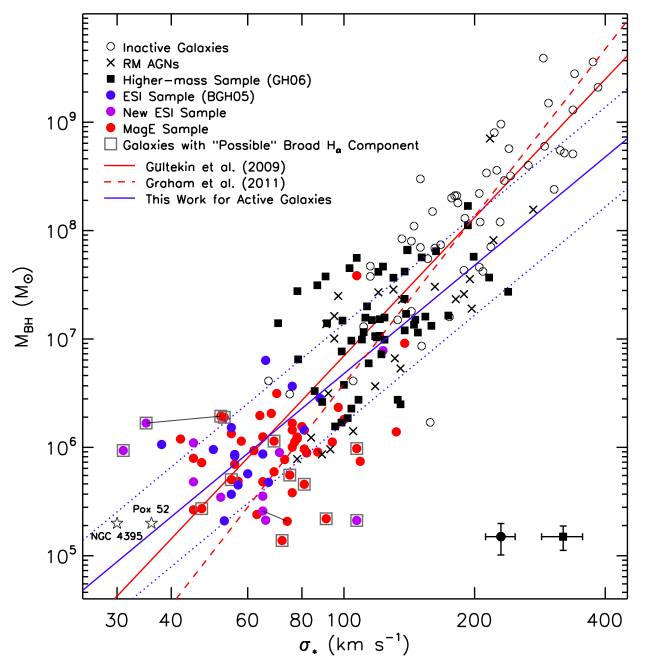
\includegraphics[angle=0]{fancymsigma}}}
%\caption[M-$\sigma$ Relation]{The M-$\sigma$ relatpion which depicts the strong correlation between the mass of a central SMBH and the velocity dispersion of its host's stellar population \citep{Xiao2011}.}
%\label{msigma} 
%\end{figure}
% Cite: Xiao

The black hole mass-bulge luminosity relation was implied by the work of \cite{Dressler1988} and first illustrated by \cite{Kormendy1993}. A wealth of evidence continues to relate these two characteristics, and follow up examinations using HST observations have determined the current, best estimates yield a M$_{\rm BH}$/M$_{\rm bulge}$ fraction between about 0.0013 and 0.0023 \citep{Merritt2001a,McLure2001,Marconi2003}. 

Major mergers between massive galaxies are thought to be efficient fueling mechanisms for bright AGN. The large influx of material due to tidal torques from the merger causes bursts of star formation and helps funnel gas directly into the center where the SMBH resides \citep[e.g.][]{Richards2006,Reddy2008,Hopkins2010}. Additionally, the most massive, highest-luminosity AGN (i.e. quasars) reside in incredibly luminous infrared galaxies where star formation is abundant, signifying that major mergers may have recently occurred \citep{Treister2012}. Distorted morphologies are often characteristics of quasar hosts, and companions can also be present around quasars, both of which are evidence that strengthen the possibility of a recent merger having affected their lifetimes. 

In many less massive and less luminous AGN, however, there is a clear lack of distorted morphologies, close neighbors, and/or other obvious merger evidence \citep{Ryan2007,Schawinski2011,Ellison2013,Hicks2013}. It is also important to note that many of these AGN exist in spiral galaxies, which are unlikely to have been recently disturbed by major mergers \citep{Springel2005,Kocevski2011}. Nevertheless, some evidence suggests \citep{vanGorkom1997,Governato2009} that disturbed galaxies may reform a disk quickly, even after a major merger as long as it is gas-rich. More recently, \cite{Treister2012} has suggested that only the highest luminosity AGN require fueling via major mergers; $\sim$90\% of AGN across all redshifts are fueled by various other mechanisms which may include minor mergers, flybys, and smooth accretion, whereby gas is directly accreted via large filaments from the ambient intergalactic medium \citep{Cox2006,Bellovary2013,Sinha2012}. 

Smooth accretion, in particular, may play an important role in fueling these low mass galaxies. Halos less than 10$^{11}$ $M_{\odot}$ can accrete filaments of unshocked gas; thereafter, gas will shock heat to the virial temperature of the halo \citep{Keres2005}. Even for massive halos, unshocked gas may still penetrate shocked regions to fuel the galaxy \citep{Brooks2007,Dekel2009,Nelson2013}. In addition, SMBH feedback, the depositing of energy and angular momentum back into the gas resevoir during accretion, also affects the overarching structure of the host galaxy \citep{Governato2009a}. Secular processes, including bar formation and disk instabilities, may also be prominent forms of accretion for these SMBHs \citep{Kormendy2013}. 

\textcolor{violet}{
It is clear that galaxy hosts grow through a variety of channels that depend on mass, environment, and interaction history. Therefore, we want to understand how these different galaxy evolutionary paths translate into SMBH fueling mechanisms, and see how they affect the fueling gas flowing into the SMBH itself. \cite{Bellovary2013} compared simulations of three high mass, high redshift galaxies and found that while mergers and smooth accretion both efficiently build up galaxies, no particular method was more adept at feeding the SMBH. Using a similar method as \cite{Bellovary2013}, this work examines the SMBH and galaxy fueling mechanisms of a Milky Way (MW) mass galaxy with a rich merger history. MW-type galaxies host SMBHs on the order of 10$^6$ $M_{\odot}$, which are likely the most common type of massive black hole, yet little is known about them or how they may grow \citep{Kormendy2013}. Through this examination, we hope to better understand the coevolution of SMBHs and their hosts in this class of galaxy. 
}

\textcolor{violet}{
In this study, we analyze the Milky Way-type galaxy, h258 [Need a face on image of ChaNGa h258](Figure \ref{h258face}), which has a history characterized by major mergers. Since this galaxy is similar to the MW in virial mass, stellar mass, and circular velocity, without a deeper examination, we may not recognize the turbulent history that it results from. We will examine the origins of gas entering the SMBH and halo to look for clues about SMBH fueling within this galaxy. By examining its assembly, and its SMBH's fueling, we can determine the accretion rate and gain further understanding about how SMBHs grow in galaxies like our own.
}

% ####### END OF INTRODUCTION #########
% #####################################


% #####################################
% ####### SIMULATION PARAMETERS #######
% #####################################

\section{Simulation Parameters}\label{sec-model}

% [NOTE TO SELF: Make/include merger trees. Ask Christina?] Can not do easily with current version parameters (halo switch turned off)
\textcolor{violet}{
Using the smoothed particle hydrodynamics (SPH) N-body tree code: Charm N-body GrAvity solver, ChaNGa, an initial DM-only, uniform resolution 50 comoving Mpc box determined what halo would be selected for zoom-in examination, including the halo examined in this paper. The DM-only simulation assumed a WMAP Year 3 cosmology \citep{Spergel2007} with the following specifications: $\Omega _m$ = 0.24, $\Omega _{\Lambda}$ = 0.76, $H_0$ = 73 km/s, and $\sigma _8$ = 0.77. The halo h258 was chosen for its Milky Way-mass, 8.6 $\times$ 10$^{11}$  M$_{\odot}$, at z=0 and its active merger history. The halo has a virial mass defined relative to a critical density, $\rho _c$, where $\rho / \rho _c$ = 100 where h258 has virial mass of $M_{\rm vir} = 7 \times 10^{11} M_{\odot}$. A recent major merger characterizes the h258 halo at z=1. This ``zoom-in'' high resolution simulation was run on this galaxy and includes gas and star particles using the volume renormalization of \cite{Katz1993}, resimulating only a few virial radii from the main halo at the highest resolution. The simulation was run from z=150 to z=0.  
}

%\subsection{High Resolution CHANGA Simulations}
\textcolor{violet}{
While a previous, low resolution version of h258 was run using the Gasoline code, this newer, high resolution version of h258 includes the following properties: a spline force softening length of 174 pc and initial gas particle masses of $2.7 \times 10^4 M_{\odot}$. Star particles are created with 30\% of their parent gas particle mass, allowing a maximum initial mass of 8100 $M_{\odot}$. Each galaxy contains about 5 million DM particles inside the virial radius at z=0 and over 14 million DM, star, and gas particles total. The resolution of both force and mass in these simulations is comparable to the ``Eris'' simulation which has one of the highest resolutions for an N-body+SPH cosmological simulation of a Milky Way-mass galaxy so far produced.  At z=9, a uniform UV background is applied to simulate the cosmic reionization energy in a variation of \cite{Haardt2012}.
}
\textcolor{violet}{
Gas can reach a minimum temperature of $\sim$100 K, in the absence of cooling via molecular hydrogen or metals. The simulation includes stochastically-modeled star formation, and once the density threshold and temperature satisfy conditions for star formation (10.0 amu cm$^{-3}$; T \textless 10$^4$ K), gas particles are eligible to form stars with an efficiency of c$^*$ = 0.1. Star particles form along the Kroupa initial mass function \citep{Kroupa2001}. Supernova feedback releases $10^{51}$ ergs of thermal energy and affects a ``blastwave'' radius determined by the equations of \cite{Ostriker1988}. In the affected region, cooling turns off for a time relative to the expansion phase of the SN remnant also determined by the blastwave equation. SN Ia and II from \cite{Thielemann1986} and \cite{Woosley1986} are adopted, respectively, and implemented through the \cite{Raiteri1996} method, which uses the stellar lifetime calculations of the Padova group \citep{Alongi1993, Bressan1993, Bertelli1994} to describe stars with varying metallicities. Both the supernova ``blastwave'' radius and supernova (Ia and II) prescriptions are described in detail by \cite{Stinson2006}. A low-temperature extension to the cooling curve is used to trace metals \citep{Bromm2001}. Simulated galaxies are shown to conform with the observed Tully-Fisher relation \citep{Governato2009}, the size-luminosity relation \citep{Brooks2011}, and the mass-metallicity relation \citep{Brooks2007}, in addition to having realistic matter distributions and baryon fractions \citep{Governato2009a,Guedes2011}. Parameter and resolution choices described above allow the galaxies to adhere to the stellar-mass-halo-mass relation at z=0 and maintain a realistic period of star formation \citep{Moster2010,Munshi2013,Brooks2007,Maiolino2008}. Given the strict adherence of this simulated galaxy with observations, we are confident that it reasonably represents growth in the galaxy and its SMBH. We exclude AGN feedback in these small to moderate mass-galaxies; however, we have determined that has little effect on the global properties of the galaxy and SMBH.
}
 
Since there are uncertainties in the formation of black holes ``seeds,'' we implement a BH seeding method that is broadly consistent with several theories of direct collapse black holes \citep{Couchman1986, Abel2002, Bromm2004} and Population III stellar remnants \citep{Loeb1994, Eisenstein1995, Koushiappas2004, Begelman2006, Lodato2006}. While this method allows the BH formation process to remain physically motivated, BH seeds form if their parent gas particle matches the criteria required for star formation and also maintains zero metallicity (2.5 amu cm$^{-3}$; T \textless 10$^4$ K; Z = 0) \citep{Stinson2006}. A probability of $\chi_{\rm seed}$ $\sim$ 0.01 is applied to determine whether a gas particle (with the above specifications) will become a BH seed with a mass of M$_{\rm BH}$ = 2.28 $\times$ 10$^5$ M$_{\odot}$, the same mass as its parent gas particle. This probability was chosen to match the predicted occupation fraction of BH seeds at z $\sim$ 3 \citep{Volonteri2008}.

The requirement that BH seeds must form from zero metallicity gas particles also causes BH formation to be constrained in areas of early star formation bursts, where the earliest and most massive halos are expected to form in the simulation. BH formation is dependent only on local environment, neglecting any large-scale properties of the host halo. Black holes are not fixed within the center of their host, allowing them to be dynamically affected by mergers and other perturbations within the galaxy. Nevertheless, BHs remain near their host centers by choosing dark matter particle masses in high-resolution regions to be on the same order as gas particle masses, minimizing two-body interactions \citep{Bellovary2011}.

Black hole mergers occur when they are separated by less than twice the softening length, and must be bound or satisfy $(1/2) \delta v^2 < \delta a \cdot \delta r$,  where $\delta v$ and $\delta a$ are the velocity and acceleration differences between the two black holes and $\delta r$ is the distance separating them. In addition to gaining mass via merger, black holes gain mass through Bondi-Hoyle gas accretion:
\begin{equation}
\dot{M} = \frac{4 \pi \alpha G^2 M^{2}_{\rm BH} \rho}{(c^{2}_{s} + v^2)^{3/2}},
\end{equation}
where $\alpha$ is a constant equal to 1, $\rho$ is the density of the surrounding gas, $c_s$ is the sound speed, and $v$ is the black hole's relative velocity to the gas. Feedback is applied to surrounding gas with an energy boost determined by the accreted mass as follows: $\dot{E}$ = $\epsilon _{r}$$\epsilon_{f}$$\dot{M}$$c^2$ where $\dot{M}$ is the accreted mass, and $\epsilon _r = 0.1$ and $\epsilon _f = 0.03$ are assumed for the radiative efficiency and feedback efficiency, respectively. This energy is distributed as thermal energy to the 32 nearest particles via a kernal probability function. Though other groups use a higher value for this efficiency, $\epsilon _f = 0.05$ \citep{Sijacki2007,DiMatteo2008}, we find that $\epsilon_f = 0.03$ in our code produces MBHs in better agreement with MBH-host galaxy scaling relations. However, as our main concern is in the relative proportion of gas in various phases, our results are not sensitive to our choices of $\epsilon _{r}$ or $\epsilon_{f}$.

\textcolor{violet}{
Compared to the previous h258 simulation, the ChaNGa simulated h258 scales better and includes a new improved SPH formalism \citep{Keller2014}. The hydrodynamic treatment now includes a geometric density average\textemdash (P$_i$ + P$_j$)/($\rho_i \rho_j$) rather than P$_i$/$\rho_{i}^2$ + P$_j$/$\rho_{j}^2$ where P$_i$ and $\rho_i$ are the particle's pressure and density\textemdash in the force expression, in addition to the standard SPH density estimator \citep{Ritchie2001}. Adjusting the force expression diminishes tensions in the numerical surface due to shear flows, such as Kelvin-Helmholtz instabilities. We also apply a consistent and entropy-conserving energy equation to account for the modified force expression and correctly model strong shocks, such as Sedov blasts. 
}

%[Talk to Glenna about Ritchie Thomas forces]

% ### END OF SIMULATION PARAMETERS ####
% #####################################


% #####################################
% ######### REDUCTION METHOD ##########	
% #####################################

\section{Reduction Method}\label{redux}

\textcolor{violet}{
The Amiga Halo Finder identifies and sets the virial radii in a simulation using an overdensity criterion for a flat universe \citep{Knebe2001,Knollmann2009,Gill2004}. We select the primary halo to be the most massive galaxy at z=0 and locate the central SMBH. For this simulation, the primary halo in h258 had a final mass on the order of $10^{12} M_{\odot}$ and a formation redshift of z$\sim$4.  
}

In this analysis, we retrace each gas particle that was accreted by the galaxy or SMBH, following the gas back through its journey in the galaxy and recording its host halo and time of accretion \citep{Brooks2009}. The particles are then classified into types by their method of entrance into the primary halo. In particular, gas particles that exist in the primary halo at the first time step are classified as ``early'' gas. Gas that belonged to a different halo than the primary prior to accretion is classified as ``clumpy,'' entering the primary halo through mergers. All other gas is classified as ``smooth'' accretion, and is then subdivided into two categories: ``cold'' and ``shocked.'' Cold or unshocked gas will usually flow into the halo via large-scale, dark matter filaments \citep{Bellovary2013}. It's possible for cold gas to be dense enough to pierce an already developed shock, allowing it to funnel into the galaxy core where it can be accreted onto the SMBH.

However, as we discussed in Section 1, if the galaxy halo is $\gtrsim$ 10$^{11}$ M$_{\odot} $, the gas is known to shock heat up to the virial temperature of the halo. We identify shocked particles through an increase in entropy and temperature using the following criteria:
\begin{equation}
T_{\rm shock} \geq 3/8 T_{\rm vir},
\end{equation}
where T$_{\rm vir}$ is the virial temperature of the halo and T$_{\rm shock}$ is the temperature of the gas particle, and 
\begin{equation}
\Delta S \geq S_{\rm shock} - S_0,
\end{equation}
where S$_0$ is the initial entropy of the gas particle, and 
\begin{equation}
S_{\rm shock} = log_{10}[3/8 T_{\rm vir}^{1.5}/4 \rho_0],
\end{equation}
where $\rho_0$ is the gas density prior to the shock. Since our halos are $\sim$ 10$^{12}$ M$_{\odot} $ by z = 0, we should expect to find more shocked gas entering the halo.

Once all the gas particles have been individually categorized, we can use these labels to determine which particles are accreting onto the SMBH, and we can better contrast the methods that feed the galaxy and its SMBH in MW-mass halos.

% ###### END OF REDUCTION METHOD ######
% #####################################


% #####################################
% ############# RESULTS ###############
% #####################################

\section{Results} \label{results}

% ########## HI RES H258 ############
%\subsection{ChaNGa - High Resolution h258}

%Just as we found in the same galaxy, h258, of the lower resolution simulation, the high resolution h258 galaxy sees a distinct preference for accreting gas that has been gained through the many mergers in its history. In this version,

\textcolor{violet}{
The galaxy h258 is characterized by two major mergers; the first occurs at z $\sim$ 1.8 and the second at z $\sim$ 1.2. Despite its merger-rich history, gas accretion can be seen smoothly increasing the cumulative black hole mass throughout its evolution (Figure \ref{hrh258allmassgas}) Figure \ref{hrh258allmassgas} shows the cumulative SMBH mass in h258 as a function of time (lower axis) and redshift (upper axis). The black dashed line indicates the total cumulative BH mass (including both mass from gas and BH mergers), while the black solid line indicates the total accreted gas mass. The blue dot-dashed line represents the gas mass accreted via unshocked gas, while the green solid line and red dashed line show the gas mass accreted through mergers and shocked gas, respectively. It is also worthwhile to point out that the largest part of the mass budget at high redshift is not gas at all, but other black holes that have merged with the SMBH seed. This has important implications for gravitational wave astronomy, increasing the event rate for SMBH assembly at high redshifts \citep{Holley-Bockelmann2010}. Aside from this early BH assembly, the largest gain in SMBH mass comes from gas associated with the major mergers between z $\sim$ 2 and z $\sim$ 1. It's clear from Figure \ref{hrh258allmassgas}, that unshocked gas makes up the majority of gas entering the galaxy at early times. However, the transitions between when smooth, unshocked accretion and mergers dominate is clearly distinguished. While clumpy gas (green) dominates at the earliest time, unshocked gas (blue) overtakes it for a short time ($\sim$ 2 Gyr) before clumpy gas once again dominates by z $\sim$ 1.5. 
}
\textcolor{violet}{
This low redshift transition to a clumpy gas preference results in the large fraction of clumpy gas seen in the SMBH (Figure \ref{hrh258stackfrac}). Figure \ref{hrh258stackfrac} depicts the fractions of total gas in the galaxy (a) and the SMBH (b) at z=0, again differentiated by gas origin. Blue, green, and red distinguish cold, clumpy, and shocked, respectively. The galaxy has a mass nearly half comprised of gas entering the galaxy through mergers (56 \%), with 36 \% of the gas entering through unshocked, smooth accretion. The smallest fraction of the total gas is comprised of shocked gas (8 \%). Unlike the galaxy, nearly three quarters of the gas accreted by the central SMBH was gas accreted via mergers, while only a quarter (24 \%) is comprised of unshocked, smoothly accreted gas. Shocked gas makes up the last 2 \% of total gas entering the SMBH. \textbf{It is evident then that the SMBH more readily accretes gas gained through mergers.} This result is contrary to \cite{Bellovary2013} which found that the fractions of gas comprising the SMBH and its host were nearly the same. Through our results, we find that lower mass galaxies can readily employ the physical effects of mergers to feed their SMBH.
}

\textcolor{violet}{
To better understand the apparent preference for merger-accreted gas, we examine the angular momentum of each type of gas at the moment it enters the galaxy. Figure \ref{hrh258angmom} shows that gas entering the SMBH (dashed lines) has an overall lower angular momentum than gas entering galaxy (solid lines), as expected; this statement is true regardless of the gas state. 
}

\textcolor{violet}{
Figure \ref{hrh258angmom_merger1} explicitly shows that at the time of the first merger, the lowest angular momentum gas entering the galaxy (solid lines) is merger-driven (green, solid line). This is reflected in the SMBH (green, dashed line) as nearly all the clumpy gas at this time funnels directly into the SMBH.
}

\textcolor{violet}{
To better understand the apparent preference for merger-accreted gas, we examine the angular momentum of each type of gas at the moment it enters the galaxy. Figure \ref{hrh258angmom} shows a cumulative distribution of the gas particles' angular momentum as they enter the halo. The gas is again distinguished by their origin (Clumpy, cold, shocked being green, blue, and red, respectively.)and between gas that ends up in the SMBH (dashed line) or the galaxy (solid lines) at z=0. We find that the angular momentum of gas entering the SMBH is lower when comparing between types of gas. We also see that the lowest angular momentum gas is comprised of both clumpy and unshocked gas. This can be seen if we examine Figure \ref{hrh258angmom_merger2} which shows the cumulative distribution of the angular momentum of the incoming gas particles at the time of the second merger. (Colors and linestyles as in Figure \ref{hrh258angmom}.) Figure \ref{hrh258angmom_merger2} explicitly shows that the gas ending up in the SMBH enters with the lowest angular momentum. There appears to be an influx of gas with low angular momentum feeding the black hole at this timestep that is not associated with the merger occurring at z $\sim$ 1.2. This may be attributed to the prior merger at z $\sim$ 1.8 (Figure \ref{hrh258angmom_merger1}) during and after which a large influx of low angular momentum gas enters the galaxy and SMBH. (Color and linestyles as in Figure \ref{hrh258angmom}) 
}

\textcolor{violet}{
A lower resolution version of the galaxy h258 was run using the N-body code, Gasoline, like those simulations in \cite{Bellovary2013}. Despite fundamental differences in the hydrodynamic implementation and gas physics included, an analysis of this low resolution h258 results in a SMBH with the same distinct preference for accreting gas. The broad consistency between the low and high resolution simulation of the same galaxy indicates that the large scale gravitational dynamics could be main driver of the SMBH fueling in this case. We also stress that that while major mergers may not be the only physical mechanisms by which gas can be funneled into the centers of galaxies (the previous study being a strong example of this), mergers between galaxies clearly play an important role when considering the gas accretion of SMBHs.
}

% ########## END OF RESULTS ###########
% #####################################


% #####################################
% ########### CONCLUSION ##############
% #####################################

\section{Conclusion}
\textcolor{violet}{
This study examines the gas accretion onto the fully cosmological simulation of a Milky Way-size galaxy to redshift z $=$ 0, with major mergers characterizing its past. We trace the gas into the SMBH at its center and differentiate the gas accreted onto the galaxy and SMBH by origin. Gas gained through mergers is classified as ``clumpy'' gas and smoothly accreted gas is seperated into ``shocked'' and ``unshocked'' categories. Our goal is to determine what types of gas are primarily feeding the SMBH and the galaxies of this class, and to determine what effects the merger history of a galaxy may have on these processes.
}

\textcolor{violet}{
A previous study by \cite{Bellovary2013} which analyized high mass, high redshift galaxies and found the gas composition of the SMBHs mirror their host. Contrary to these previous results, when we examined a galaxy with an active merger history, we determined that the SMBH at the center more readily accretes gas gained through mergers. This remained true both in an older low resolution simulation of the same galaxy as well as this current iteration. \textbf{In both the low and high resolution cases, we see a significant increase in the clumpy gas accreted by the SMBH compared to its host.} 
}

The angular momentum of the accreted gas as it enters the galaxy sheds some light on the mechanism driving this preferentially accreted clumpy gas. Smoothly accreted gas, which enters with galaxy with a wide range of angular momentum, may become additionally torqued by the already existing disk. Meanwhile, gas entering through mergers is restricted by the direction of its entry and allows for a small range of low angular momentum gas to enter the main halo. This gives clumpy gas the advantage of falling more readily to the center and accreting onto the SMBH. Considering all origins of gas, we see a clear distinction wherein lower angular momentum gas preferentially feeds the SMBH.

\textcolor{violet}{
However, because this reult departs from the previous study, we consider that some of the physical processes affecting the galaxy with an active merger history accounts for the ready funneling of low angular momentum to the central region of the black hole. 
}
\textcolor{violet}{
While the examination of this extreme case of a galaxy with an active merger history depicts a class of galaxy with varying SMBH accretion methods, a further study of cases with varying merger histories is required to begin understanding the broad spectrum of Milky Way-mass galaxy accretion. It is clear through this study that the presence of major mergers can play an important role in the final compositions of central SMBHs, but the question of how important these mergers are remains to be seen.
}

% ####### END OF CONCLUSIONS ##########
% #####################################


\acknowledgments
Thank you to the Fisk-Vanderbilt Masters-to-PhD Bridge program for their continued funding and support of this research.
Also thank: American Museum of Natural History. N-Body shop, for use of their code? Others? [GET GRANT NUMBERS?]

%\begin{figure}
%\centerline{
 % \resizebox{0.95\hsize}{!}{\includegraphics[angle=0]{fig1a.pdf}}
  %}
%\centerline{
 % \resizebox{0.95\hsize}{!}{\includegraphics[angle=0]{fig1b.pdf}}
  %}  
  %\centerline{
  %\resizebox{0.95\hsize}{!}{\includegraphics[angle=0]{fig1c.pdf}}
  %}
%\caption[]{Evolution of our flat rotating model (A0) in isolation.
%Top Panel: Stellar density profile at various times. $\gamma = 1.0$ is the reference theoretical profile, shown as a dashed line. Middle Panel: Evolution of intermediate to major (b/a) and minor to major %(c/a) axis ratio as measured at the half mass radius. Bottom Panel: Ratio of rotational velocity to the 3-d velocity dispersion as a function of distance at various times. In isolation, the rotational support in the center decreases over time as the central SMBH increases the velocity dispersion.
%} \label{stab}
%\end{figure} 

\begin{figure}
\centerline{\resizebox{0.75\hsize}{!}{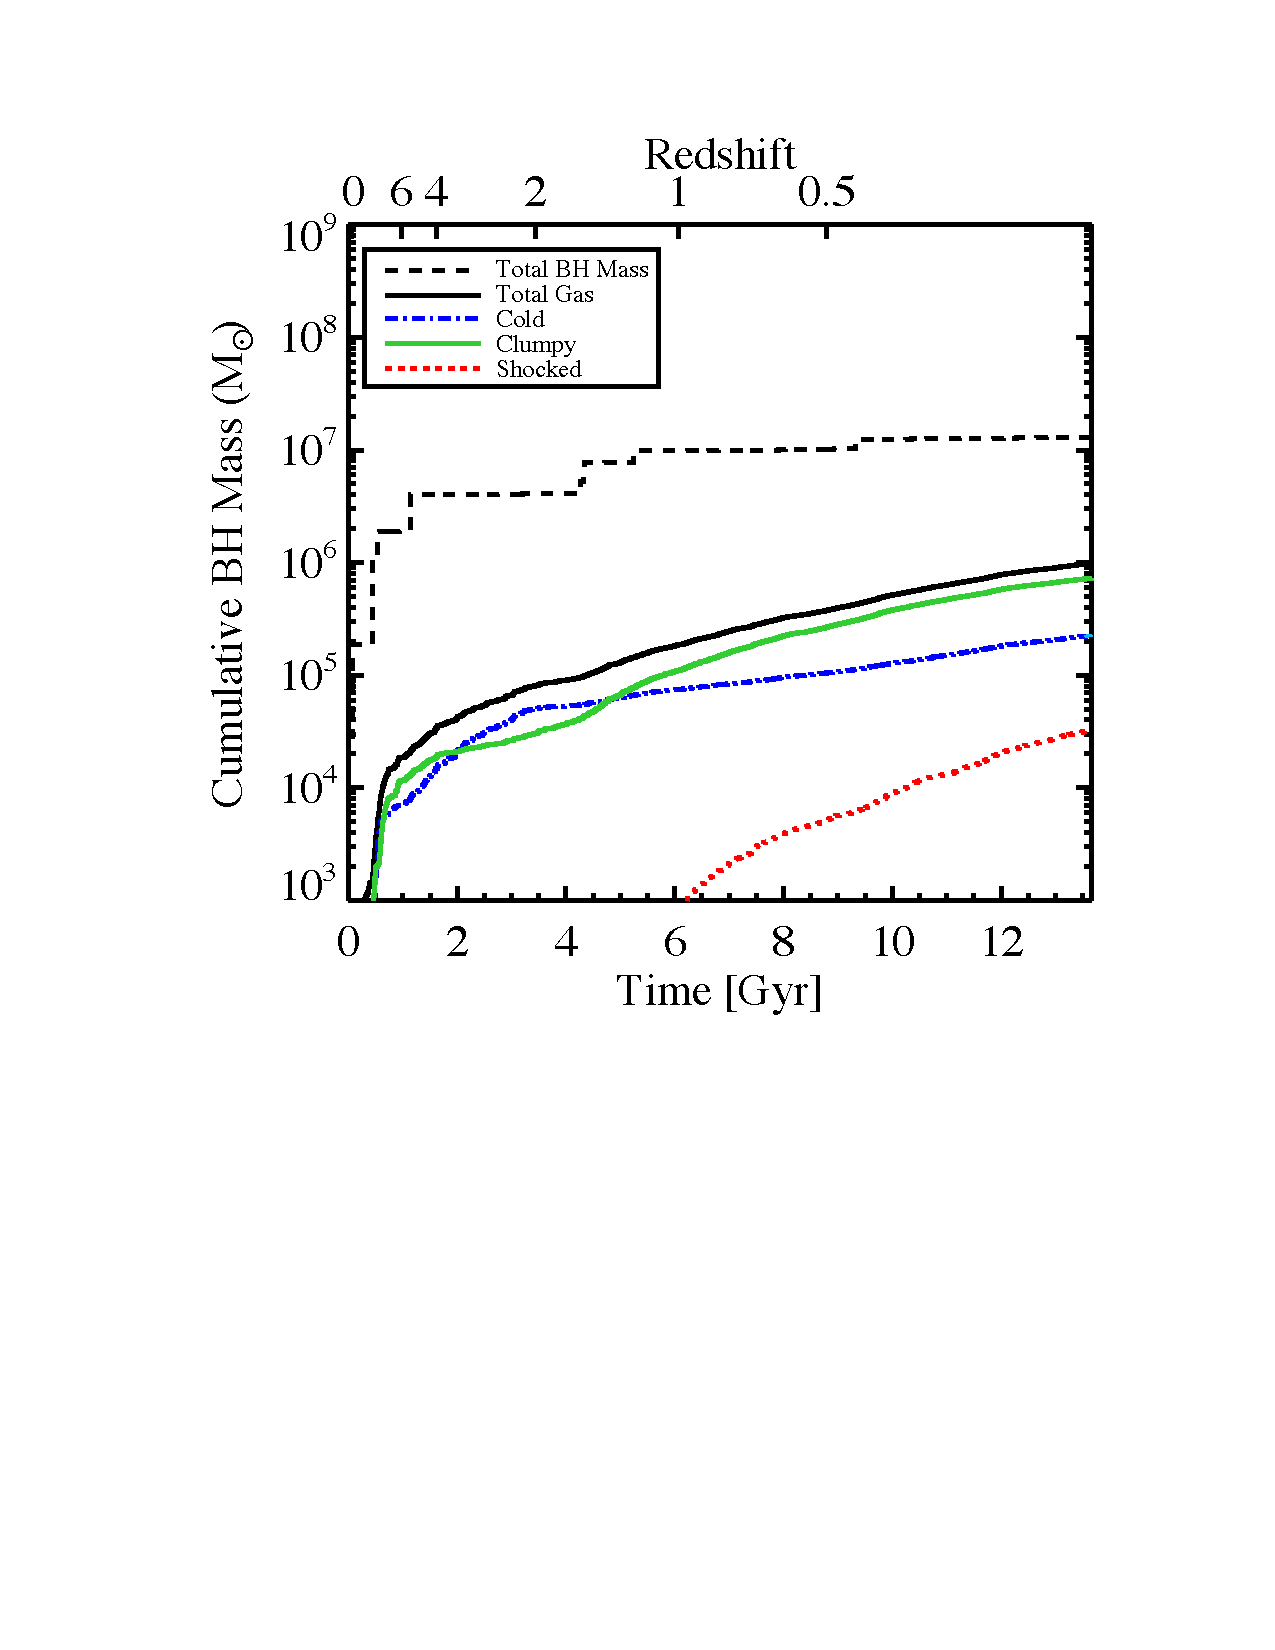
\includegraphics[angle=0]{hrh258_massgastime}}}
\caption[]{The central BH’s cumulative mass as a function of time and redshift. The black dashed line indicates the total cumulative BH mass. The black solid line indicates the total gas mass. The blue dot-dashed line indicates the gas mass accreted via unshocked gas. The green solid line indicates the gas mass accreted through mergers. The red dashed line indicates gas mass that was shocked upon entry into the halo.}
\label{hrh258allmassgas} 
\end{figure}

\begin{figure}
\centerline{\resizebox{0.75\hsize}{!}{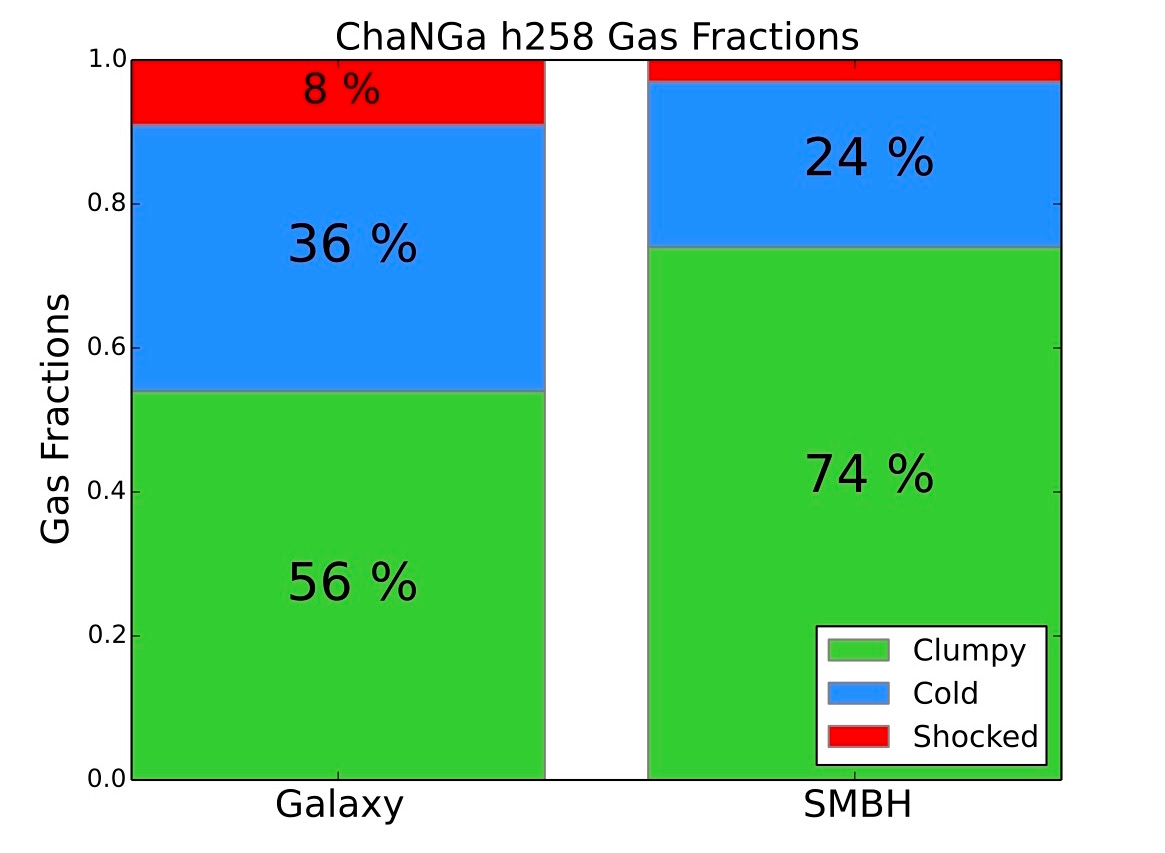
\includegraphics[angle=0]{hrh258_stackbarfractions_good}}}
\caption[]{Gas fractions of the gas particles accreted by the high resolution ChaNGA h258 by the main halo (left) and the SMBH (right), distinguished by type. Blue, green, and red distinguish gas gained through unshocked gas, gained through mergers, and gas shocked upon entry, respectively. Yellow indicates gas that existed within the main halo upon formation; this ``early'' gas is negligable ($<$ 1 \%) within the SMBH.}
\label{hrh258stackfrac} 
\end{figure}

\begin{figure}
\centerline{\resizebox{0.75\hsize}{!}{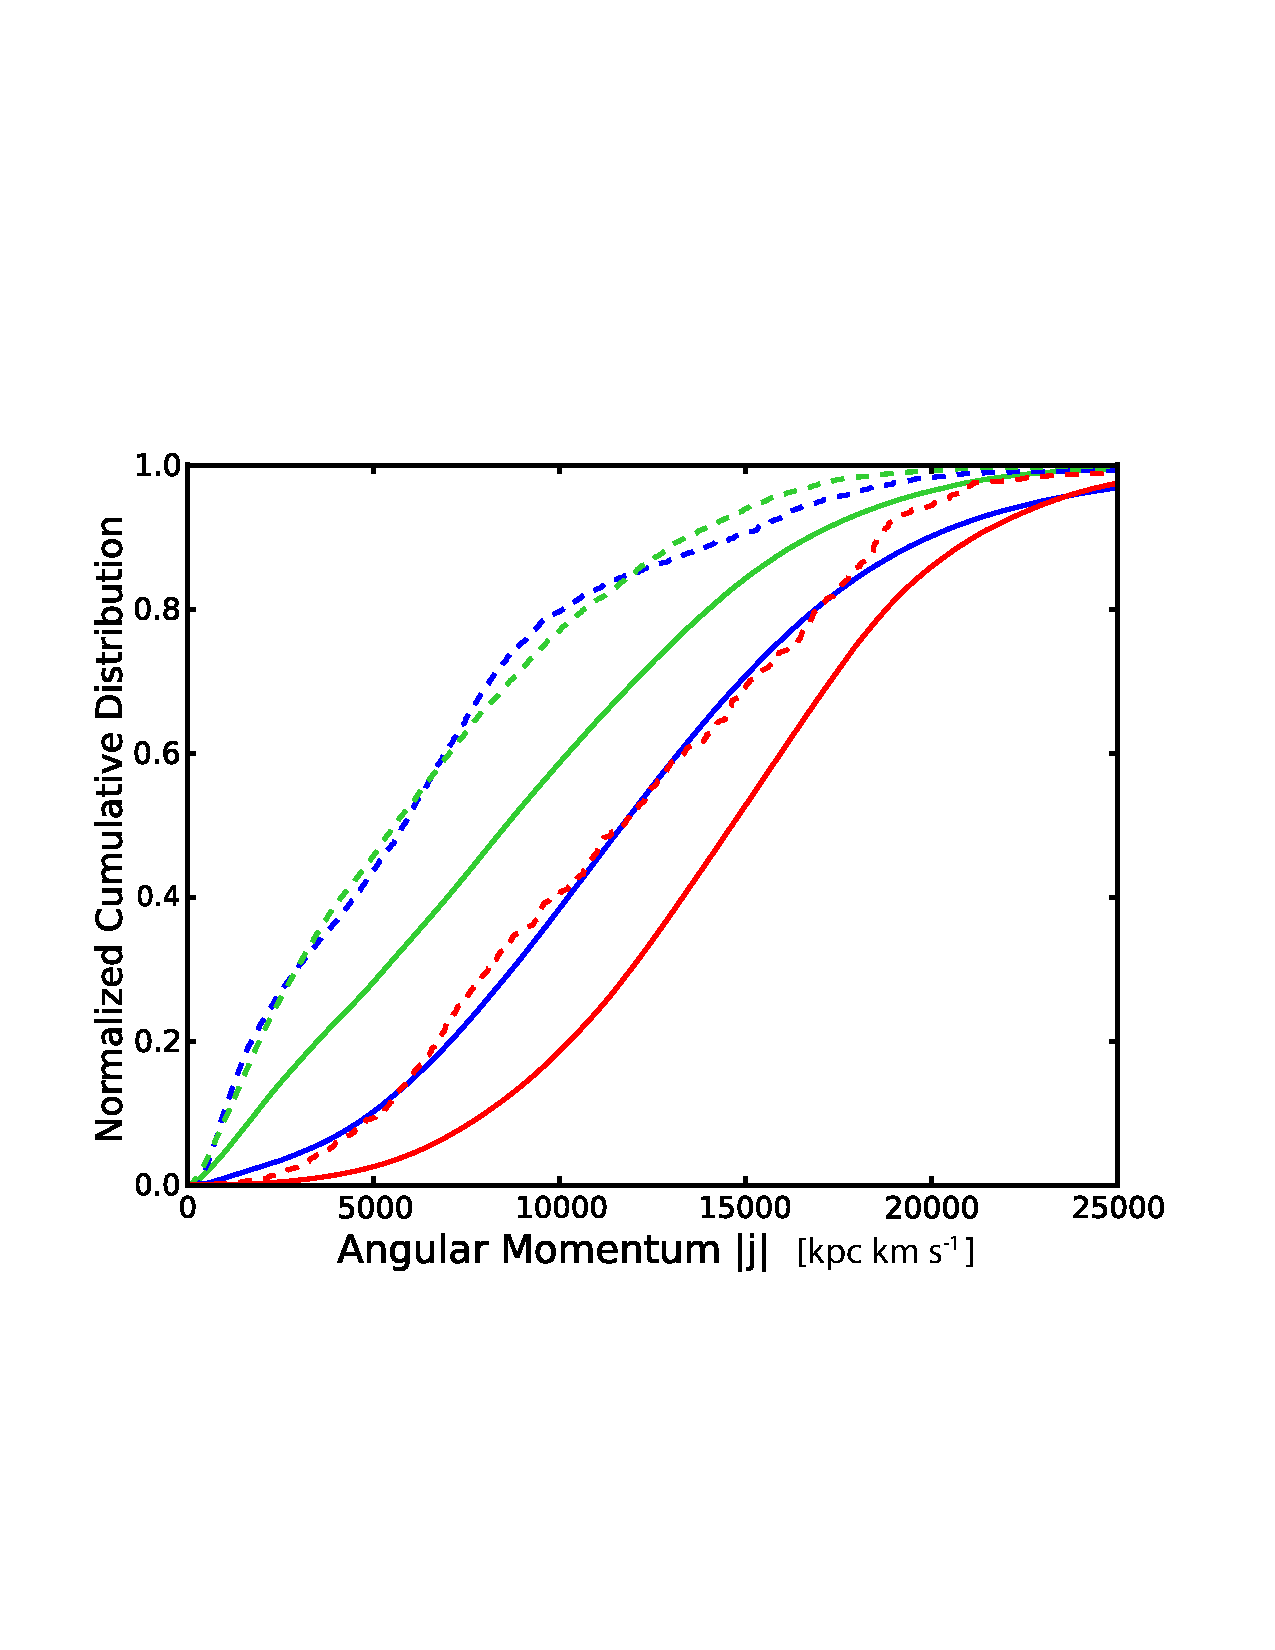
\includegraphics[angle=0]{hrh258_am_cumu_4096}}}
\caption[]{ Cumulative distribution of angular momentum of the gas particles accreted onto the high resolution ChaNGa h258.  Gas particles accreted onto the main halo (solid lines) and central black hole (dashed lines). The green, blue, and red lines indicate clumpy, unshocked, and shocked gas, respectively.}
\label{hrh258angmom} 
\end{figure}

\begin{figure}
\centerline{\resizebox{0.75\hsize}{!}{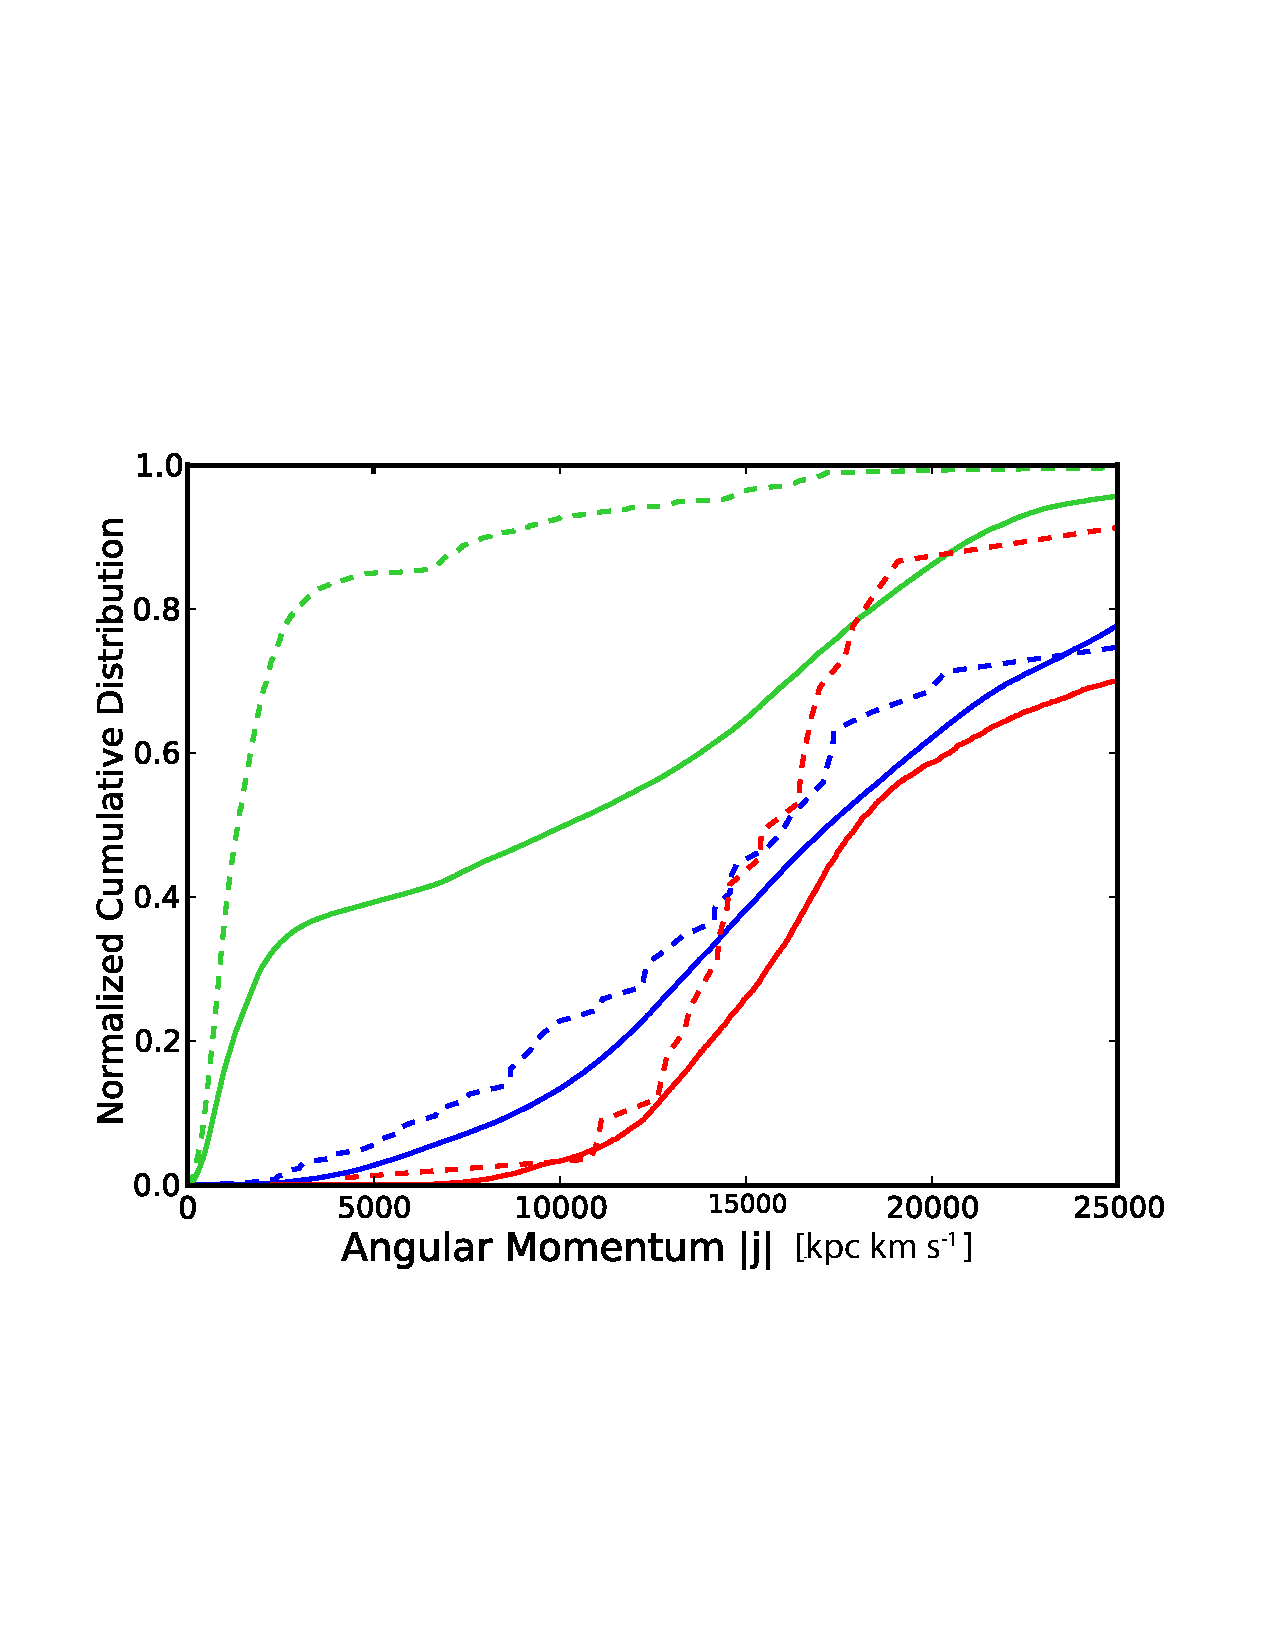
\includegraphics[angle=0]{hrh258_am_tsnew_1584}}}
\caption[]{ Cumulative distribution of angular momentum of the gas particles accreted onto the high resolution ChaNGA h258 galaxy at the time of the second major merger (z $\sim$ 1.2). There are about 450,000 gas particles accreted at this timestep, which gas particles accreted onto the main halo and central black hole are distinguished by solid and dashed lines. The green, blue, and red lines indicate clumpy, unshocked, and shocked gas, respectively.}
\label{hrh258angmom_merger2} 
\end{figure}

\begin{figure}
\centerline{\resizebox{0.75\hsize}{!}{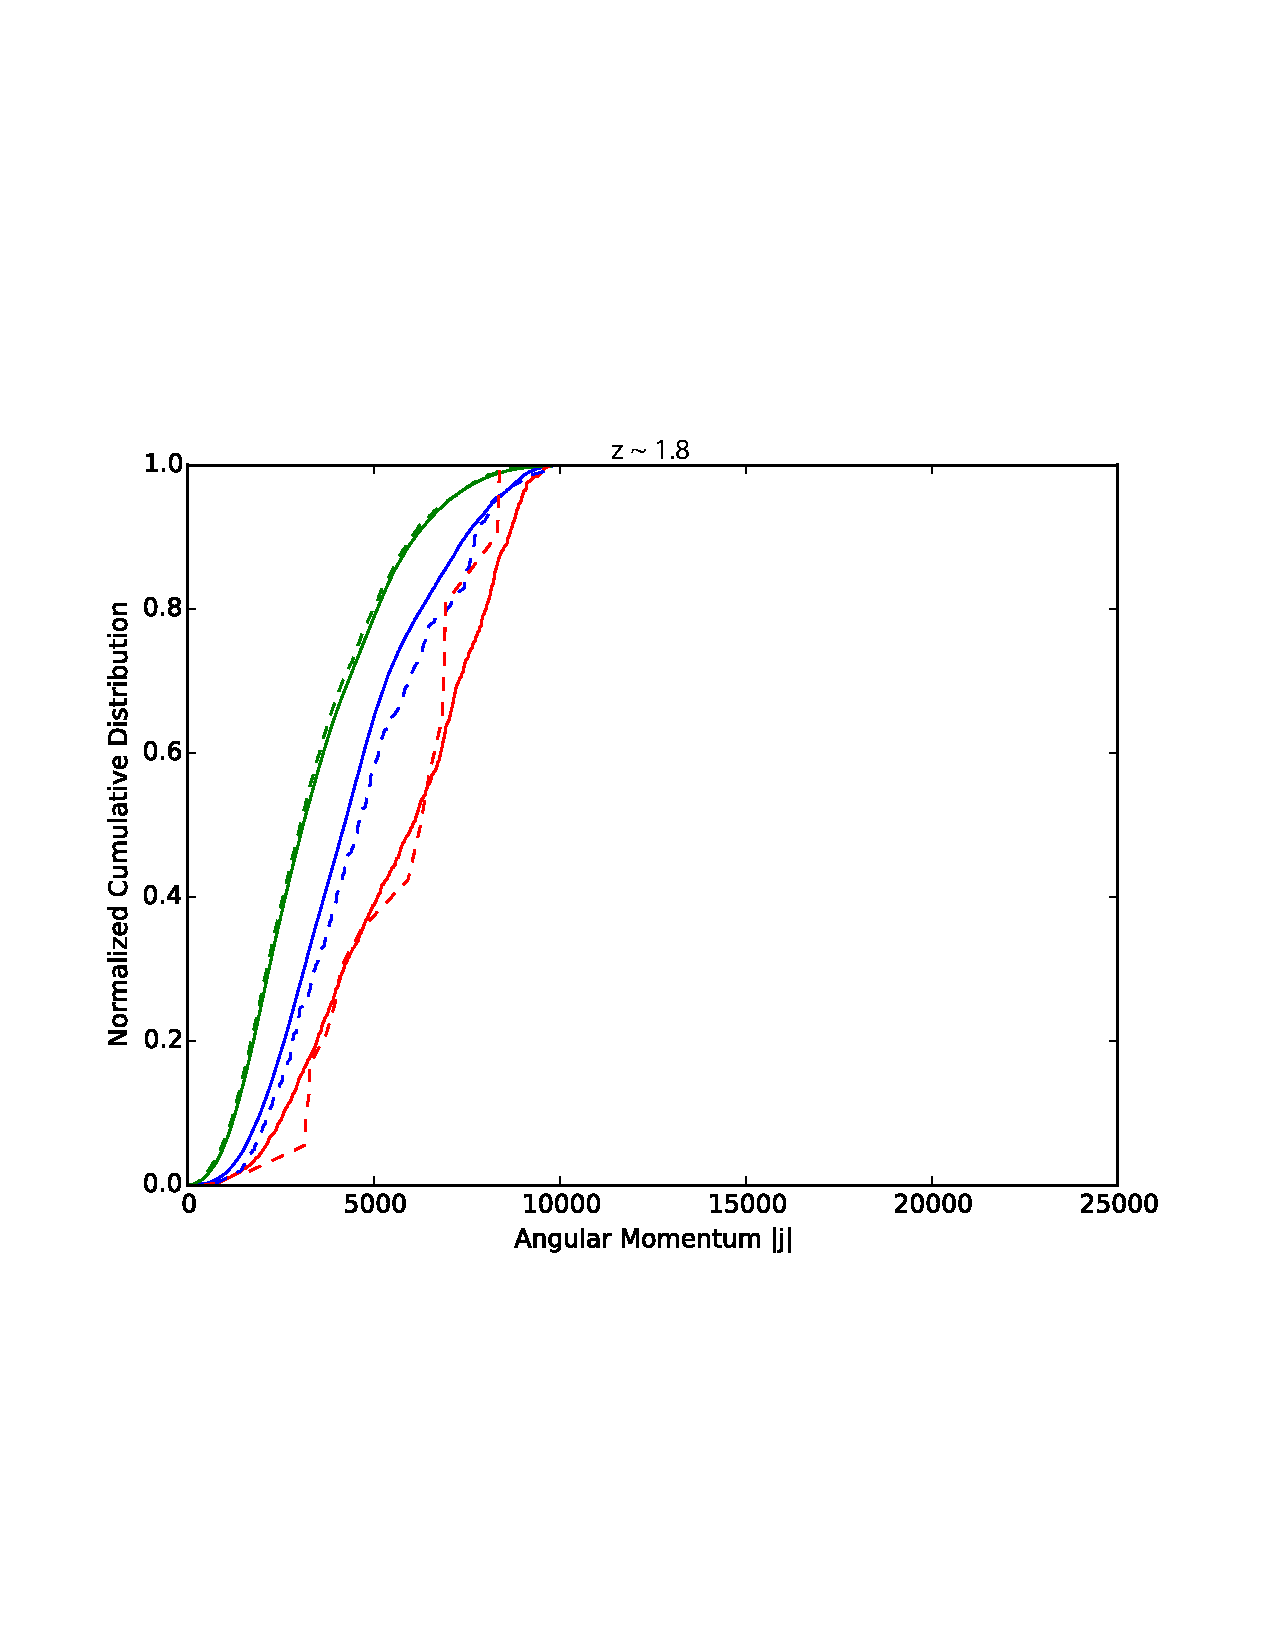
\includegraphics[angle=0]{hrh258_am_tsnew_1128}}}
\caption[]{ Cumulative distribution of angular momentum of the gas particles accreted onto the high resolution ChaNGA h258 galaxy at the time of the first major merger (z $\sim$ 1.8). There are about 900,000 gas particles accreted at this timestep, which gas particles accreted onto the main halo and central black hole are distinguished by solid and dashed lines. The green, blue, and red lines indicate clumpy, unshocked, and shocked gas, respectively.}
\label{hrh258angmom_merger1} 
\end{figure}

\bibliography{/Users/the_neekster/Documents/MENDELEY/MEND_bibtexfiles/Sanchez2016.bib}

\end{document}

